\chapter{Modern Cryptographic Definitions}


\section{The Three Principles of Modern Cryptology}

\begin{enumerate}
    \item Formulate a rigorous and \textbf{precise definition of security}.
    \item When a cryptographic system relies on an \textbf{unproven assumption}, it must be \textbf{precisely stated}. Furthermore, this assumption \textbf{must be minimal}.
    \item Cryptographic constructions must be accompanied by a \textbf{rigorous proof of security} with respect to the definition formulated in principle 1, revolving around the assumptions stated in principle 2.
\end{enumerate}

\subsection{Principle 1: Formulation of Exact Definitions}

\begin{itemize}
    \item \textbf{Why is this important?}
    \begin{itemize}
        \item \textbf{Importance for design:} We need to have a good understanding of our goal so that
we know when we achieve it. Sometimes our cryptographic system doesn't need to
be as efficient as possible, a simpler version being sufficient.
        \item \textbf{Importance for usage:} When we want to choose an existing cryptographic scheme
we need to have some sort of comparison criteria to be able to tell if it suffices our
application.
        \item \textbf{Importance for study:} For researching different types of cryptographic systems
we need to be able to compare them and measure their security level. Without
a rigorous proof of security the only performance attribute we can measure is
efficiency (which is not very accurate).
    \end{itemize}
    \item \textbf{How do we define security?}
    \begin{itemize}
        \item An encryption scheme is secure if no adversary can compute any function of the
plaintext from the cipher text.
        \item An encryption scheme is considered broken if an adversary learns some function of
the plaintext from the cipher text.
        \item The power of the adversary relates to assumptions regarding the actions the
adversary is assumed to be able to take, as well as the adversary's computational
power.
    \end{itemize}
\end{itemize}

\subsection{Principle 2: Reliance on Precise Assumptions}

Most cryptographic constructions cannot be proven secure unconditionally, therefore it relies on some assumptions which must be precisely stated for the following reasons:

\begin{enumerate}
\item \textbf{Validation of the assumption} If the assumption being relied upon is not precisely stated and presented it cannot be studied and potentially refuted.
\item \textbf{Comparison of schemes} If the assumptions used by two schemes are incomparable, then the one based on the better-studied or the simpler assumptions is preferred.
\item \textbf{Facilitation of proofs of security} A mathematical proof that ``the construction is secure if the assumption holds'' cannot be provided without a precise statement of what the assumption is.
\end{enumerate}

\subsection{Principle 3: Rigorous Proofs of Security}

The first two principles lead naturally to this one. Most proofs in modern cryptography use the \textbf{reductionist} approach, that is, \textit{``Given the Assumption A is true, Construction C is secure according to the given definition.''}

\section{Cryptographic Games}

We can capture a notion of security by a picture representing a game played with adversary $A$. The games have one of two goals and the adversary has a range of powers.

\subsection{Indistinguishability (IND-Security)}

Indistinguishability is a measure of security whereby an adversary offers you (the challenger) two messages, and if you were to encrypt only one of them, he / she would be unable to tell \textbf{which one you have encrypted}.\\
\\
Figure~\ref{fig:ind-sec-sym} shows the cryptographic game which captures this for a symmetric cryptographic scheme. $\csubm{0}$ and $\csubm{1}$ are the two messages the adversary gives you and $\ccast$ is the ciphertext you computed from one of the messages. $b'$ is the answer the adversary gives. Note that $|\csubm{0}|=|\csubm{1}|$, since a difference in size would be a dead give away.\\
\begin{figure}[htp!]
    \centering
    \begin{subfigure}[b]{0.4\textwidth}
        \centering
        \begin{cryptogame}{$b\in \{0,1\}$}
            \cgameleft{$\csubm{m},\csubm{m}$}
            \cgameright{$\ccast=\textrm{Enc}_\ck(\csubm{b})$}
            \cgameleft{$b'$}
        \end{cryptogame}
        \caption{Symmetric Key  Case}
        \label{fig:ind-sec-sym}
    \end{subfigure}
    ~
    \begin{subfigure}[b]{0.4\textwidth}
        \centering
        \begin{cryptogame}{$b\in \{0,1\}$}
            \cgameright{$\cpk$}
            \cgameleft{$\csubm{0},\csubm{1}$}
            \cgameright{$\ccast=\textrm{Enc}_{\csk}(\csubm{b})$}
            \cgameleft{$b'$}
        \end{cryptogame}
        \caption{Public Key Case}
        \label{fig:ind-sec-pub}
    \end{subfigure}
    \caption{IND-Security Games}
    \label{fig:ind-sec}
\end{figure}
\\
Figure~\ref{fig:ind-sec-pub} shows the game design for public key encryption. $\cpk$ is the publicly available key, which all adversaries would have access to while trying to crack your message.\\
\\
A cryptographic system fails a game if an adversary can win the game more often than chance (i.e. $> 50\%$ success rate).

\subsection{One-wayness (OW-Security)}

One-wayness is the property that an attacker, with only the ciphertext, \textbf{cannot decrypt the message}. The layout of the games used for this are in Figure~\ref{fig:ow-sec}.

\begin{figure}[htp!]
    \centering
    \begin{subfigure}[b]{0.4\textwidth}
        \centering
        \begin{cryptogame}{$\cm\in \mathbb{P}$}
            \cgameright{$\ccast=\textrm{Enc}_\ck(\csubm{b})$}
            \cgameleft{$m'$}
        \end{cryptogame}
        \caption{Symmetric Key  Case}
        \label{fig:ow-sec-sym}
    \end{subfigure}
    ~
    % TODO: This game is identical to public key IND-Security. Somethings not right here.
    \begin{subfigure}[b]{0.4\textwidth}
        \centering
        \begin{cryptogame}{$b\in \{0,1\}$}
            \cgameright{$\cpk$}
            \cgameleft{$\csubm{0},\csubm{1}$}
            \cgameright{$\ccast=\textrm{Enc}_{\csk}(\csubm{b})$}
            \cgameleft{$b'$}
        \end{cryptogame}
        \caption{Public Key Case}
        \label{fig:ow-sec-pub}
    \end{subfigure}
    \caption{OW-Security Games}
    \label{fig:ow-sec}
\end{figure}

\subsection{Adversarial Powers}
These attacks also have defined `adversarial powers', where the adversary has access to specific oracles.
\begin{itemize}
    \item \textbf{Passive Attack}: Has no oracles --- all games above are passive attacks.
    \item \textbf{Chosen Plaintext Attack (CPA)}: The adversary can encrypt any mesage of his/her choosing.
    \item \textbf{Chosen Ciphertext Attack (CCA)}: The adversary can decrypt any message of his choosing, except he is not allowed to decrypt $\ccast$.
\end{itemize}
We assume that if an adversary has access to a decryption oracle, then they have access to the encryption one, so CCA is an extension of CPA\footnote{Except in one case we will see later on concerning hybrid encryption schemes.}. There is no notion of a passive attack for public key encryption because the public key (which is used to encrypt) is public, so the adversary always has an encryption oracle.

\section{Reductions}
We can make comparisons of problems by reducing one to another, thereby defining one as `no harder' than the other. A reduction is where we can, in polynomial time, convert a problem into another one. We say \textbf{Problem A is no harder than Problem B} if we can convert Problem A into Problem B. This is written as \boldmath $A \leq_P B$ \unboldmath.\\
\begin{figure}[htp!]
    \begin{center}
        \begin{tabular}{ccccc}
            \gbox{IND-CCA} & $\rightarrow$ & \gbox{IND-CPA} & $\rightarrow$ & \gbox{IND-PASS}\\
            $\downarrow$ && $\downarrow$ && $\downarrow$ \\
            \gbox{OW-CCA} & $\rightarrow$ & \gbox{OW-CPA} & $\rightarrow$ & \gbox{OW-PASS}\\
        \end{tabular}
    \end{center}
    \caption{Relationships between attacks}
    \label{fig:relations}
\end{figure}
\\
Some attacks are more powerful than others. Figure~\ref{fig:relations} show these relationships between the attacks. An arrow ($A \rightarrow B$) means $A$ is more powerful than $B$ and thus a proof that a system meets $A$'s notion of security, also proves it meets $B$'s.\\
\\
\textbf{IND-CCA is the de-facto} security definition we should accept. This means that the encryption must be probabilistic (i.e. encryption is a one-to-many function) because it could ask the oracle to encrypt $m_0$ and from that could win the game.


\section{Stream Ciphers}
The idea behind a stream cipher is to replace the (possibly) huge cipher needed for the One-Time-Pad scheme by a pseudo-random sequence which is `seeded' by a key of a more practical size. There's some confusion over whether the term `stream cipher' refers to the algorithm generating the stream or the entire encryption scheme. The term can mean both, but the book accompanying the unit recommends you only use it for the algorithm.\\
\begin{figure}[htp!]
    \begin{center}
        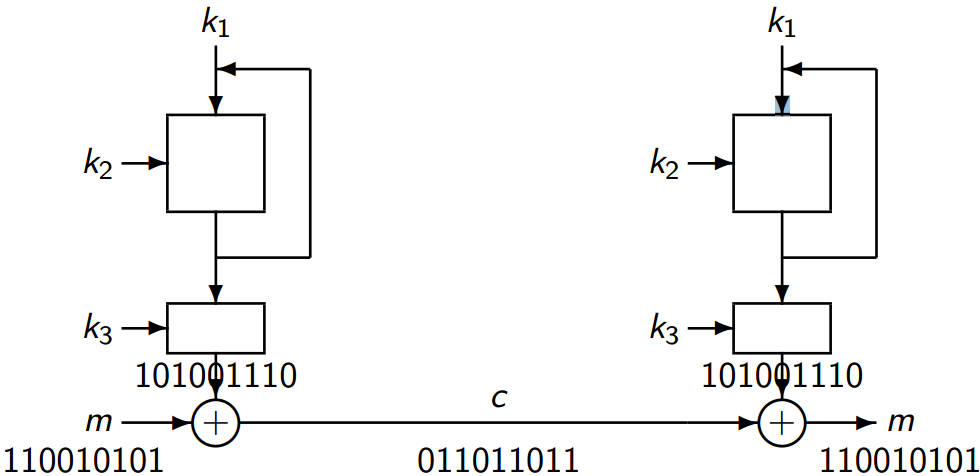
\includegraphics[width=0.7\textwidth]{img/streamcipher}
        \caption{A stream cipher using a DFA where keys determine state update ($\csubk{1}$), initial state ($\csubk{2}$) and output filter ($\csubk{3}$)}
    \end{center}
\end{figure}
\\
One model of a stream cipher is a finite state machine, where the key provides the initial state, variables used to convert a keystream, $\csubk{i}$, to the next keystream, $\csubk{i+1}$. The ouput of the FSA is also XORed with a value taken from the key.\\
\\
One source for confusion may come from that fact that the slides use $\csubk{x}$ to mean both the key values which are input into the stream cipher, and for the keystream, which is the output of the stream cipher.\\
\\
Decryption is easy as both sender and receiver use one key to generate the keystream of necessary size. This is possible because the algorithm is deterministic, which, as mentioned later, is a source of weakness.
